	\subsection{group}
This section defines the form's structure in terms of its base components: \textbf{group}s, \textbf{element}s and \textbf{item}s.

Groups hold elements (see \ref{element}) which, in turn, contain items (see \ref{item}).
Each group must have an \textit{xml:id} and it can have a label for every language it should support.

A template will be composed by one or more groups.

Attributes:
\begin{center}
	\begin{tabular}{ | p{0.2\textwidth} | p{0.7\textwidth} | }
		\hline
		Attribute & Description \\ 
		\hline
		xml:id & unique id \\
		\hline
	\end{tabular}
\end{center}

Child tags:
\begin{center}
	\begin{tabular}{ | p{0.2\textwidth} | p{0.7\textwidth} | }
		\hline
		Tag & Description \\ 
		\hline
		label & one for each xml:lang to be supported \\
		help & one for each xml:lang to be supported \\
		\hline
		element & one for each element \\
		\hline
		
	\end{tabular}
\end{center}

\begin{figure}[h]
	\caption{Group example}
	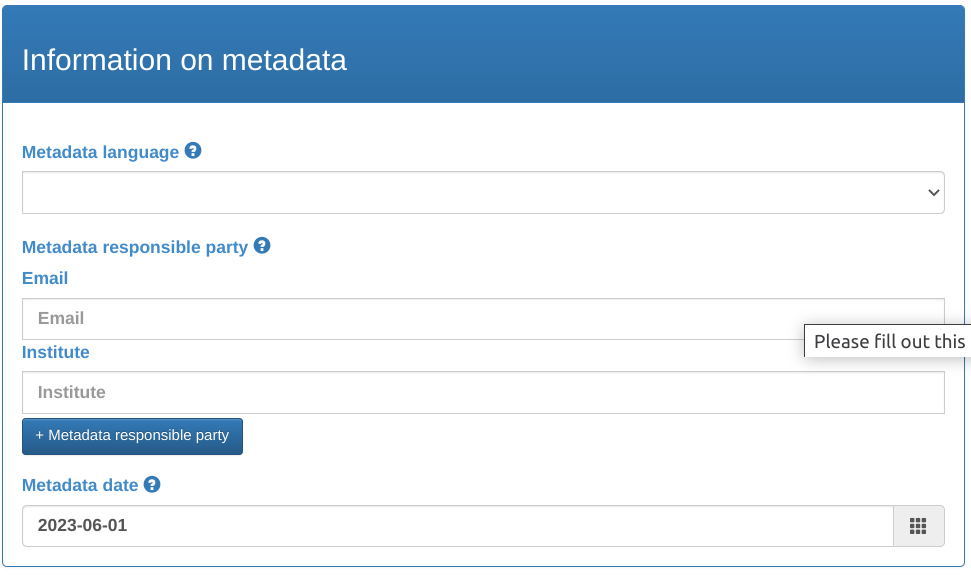
\includegraphics[width=10cm]{Group example.png}
	\centering
\end{figure}

\begin{lstlisting}[language=xml]
	<group xml:id="info_md">
	<label xml:lang="en">Information on metadata</label>
	<label xml:lang="it">Informazioni sui metadati</label>
	...
	</group>
\end{lstlisting}

\subsubsection{element} \label{element}
Elements are groupings of *item*s that share conceptual purpose and a shared root in the resulting XML.

Attributes:
\begin{center}
	\begin{tabular}{ | p{0.2\textwidth} | p{0.7\textwidth} | }
		\hline
		Attribute & Description \\ 
		\hline
		xml:id & unique id \\
		\hline
		isMandatory & \textbf{true} if all underlying items must have a value \\ & \textbf{false} otherwise \\
		\hline
		isMultiple & \textbf{true} if element can have multiple instances \\ & \textbf{false} otherwise  \\
		\hline
		alternativeTo & if present it means this element is an exclusive alternative for another item: only the one of the two that has been filled in will make it to the final XML \\
		\hline
	\end{tabular}
\end{center}

Child tags:
\begin{center}
	\begin{tabular}{ | p{0.2\textwidth} | p{0.7\textwidth} | }
		\hline
		Tag & Description \\ 
		\hline
		label & one for each xml:lang to be supported \\
		help & one for each xml:lang to be supported \\
		\hline
		hasRoot & represents the root tag in the destination XML \\
		\hline
		produces & container tag for \textit{items} \\
		\hline
		
	\end{tabular}
\end{center}

\begin{figure}[h]
	\caption{Element example (single item)}
	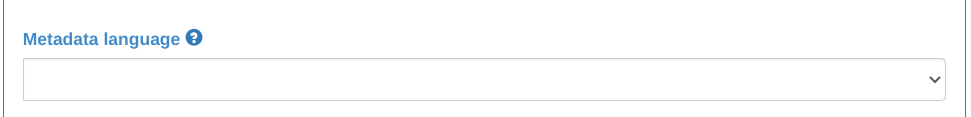
\includegraphics[width=10cm]{Element single item.png}
	\centering
\end{figure}

\begin{lstlisting}[language=XML]
	<element xml:id="id_md" isMandatory="true" isMultiple="false">
	<label xml:lang="en">File identifier</label>
	<label xml:lang="it">Identificatore del file</label>
	<help xml:lang="en">The element must contain, as a prefix, the iPA code assigned by 
	the Administration in the Index of Public Administrations (e.g., "cnr:112358").</help>
	<help xml:lang="it">L'elemento deve contenere, come prefisso, il codice iPA assegnato
	all'Amministrazione nel momento dell'accreditamento all'Indice delle Pubbliche
	Amministrazioni (es. "cnr:112358").</help>
	<hasRoot>/gmd:MD_Metadata/gmd:fileIdentifier</hasRoot>
	<produces>
	<item hasIndex="1" xml:id="id_md_1" queryStringParameter="uid" isFixed="true" hasDatatype="string">
	<hasPath>/gmd:MD_Metadata/gmd:fileIdentifier/gco:CharacterString</hasPath>
	</item>
	</produces>
	</element>
\end{lstlisting}

\begin{figure}[h]
	\caption{Element example (multiple items)}
	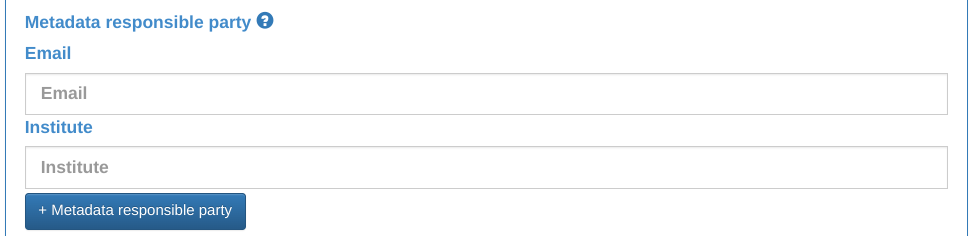
\includegraphics[width=10cm]{Element multiple items.png}
	\centering
\end{figure}


\paragraph{item} \label{item}

Attributes:
\begin{center}
	\begin{tabular}{ | p{0.3\textwidth} | p{0.6\textwidth} | }
		\hline
		Attribute & Description \\ 
		\hline
		xml:id & unique id \\
		\hline
		hasIndex & a string representing the index of this item in the order of shown items inside the element \\
		\hline
		outIndex & a string representing the index of this item in the order required inside the element XML representation \\
		\hline
		hasDatatype & data type of the item: must be one of the \hyperref[datatypes]{supported data types} \\
		\hline
		isFixed & \textbf{true}: the item is neither visible nor editable \\
		& \textbf{false}: the item is visible and editable \\
		\hline
		hasPath & the destination path in the XML output document: it can be relative relative to the hasRoot attribute of containing element \\
		\hline
		datasource & optional datasource id holding allowed values \\
		\hline
		field & optional field holding the allowed value \\
		\hline
		isLanguageNeutral & optional indication to instruct EDI Client to use language neutral results from a datasource, overriding the default metadata language \\
		\hline
		defaultValue & optionally used to 		specify a default value for the item \\
		\hline
		useCode & optionally specifies that the code (URI or urn) field should be used from the datasource \\
		\hline
		show & (\textbf{TODO: check if really implemented}) optionally override default control used as input with a specific one \\
		\hline
		queryStringParameter & if specified, it allows the initial value of this item to be specified in the query string: the value of this attribute defines the key / value pair in the query string \\
		\hline
	\end{tabular}
\end{center}

Child tags:
\begin{center}
	\begin{tabular}{ | p{0.2\textwidth} | p{0.7\textwidth} | }
		\hline
		Tag & Description \\ 
		\hline
		label & one for each xml:lang to be supported \\
		help & one for each xml:lang to be supported \\
		\hline
		hasRoot & represents the root tag in the destination XML \\
		\hline
		produces & container tag for \textit{items} \\
		\hline
		
	\end{tabular}
\end{center}

